\chapter{Сравнительный анализ существующих алгоритмов и реализаций}    

\section{Общие теоретические положения}   

Человек может сравнить изображения и выделять на них объекты визуально, на интуитивном уровне. Однако, для машины изображение — всего лишь ни о чем не говорящий набор данных. Одной из больших проблем в сопоставлении изображений является очень большая размерность пространства, по которому "размазана" информация. Если взять картинку размером хотя бы $100*100$, то уже получим размерность равную $10^4$. Как же компьютер обретает зрение?

Основная идея состоит в том, чтобы получить какую-то характеристику, которая будет хорошо описывать изображение, легко вычисляться и к которой можно применить логическую операцию сравнения. Эта "характеристика" должна быть устойчива к различным преобразованиям (сдвиг, поворот и масштабирование изображений, изменения яркости, изменения положения камеры). Чтобы определять один и тот же объект на изображениях сделанных с разных углов, расстояний и при разном освещении.

Все эти условия приводят к необходимости выделения на изображении особых, ключевых точек (\textbf{key points}). Этот процесс называется \textbf{feature extraction}. Ключевая точка - эта такая особая точка, которая отличается от соседних точек и будет не похожа на остальные, соответственно является, в какой-то степени, уникальным свойством этого изображения. Таким образом машина может представить изображение как модель состоящие из ключевых точек. Примером особых точек, если говорить об изображении лица человека, могут служить глаза, уголки губ, кончик носа. 

После выделения особых точек компьютеру нужно уметь их сравнивать. Этот процесс называется \textbf{feature matching}. Для сравнения удобно использовать дескрипторы (\textbf{descriptor} - "описатель"). Дескриптор - своеобразный описатель или идентификатор ключевой точки, выделяющий её из остальной массы особых точек. Как мы увидим далее именно благодаря дескрипторам получается инвариантность относительно преобразований изображений. 
В итоге получается следующая схема решения задачи сопоставления изображений:

\begin{enumerate}
    \item На изображениях выделяются ключевые точки и их дескрипторы;
    \item По совпадению дескрипторов выделяются соответствующие друг другу ключевые точки;
    \item На основе набора совпавших ключевых точек строится модель преобразования изображений, с помощью которого из одного изображения можно получить другое;
\end{enumerate}

Далее будут подробнее рассмотрены \textbf{feature-based algorithms} (алгоритмы основанные на особых точках)

\section{Алгоритм SIFT}   

\textbf{Scale-invariant feature transform} (SIFT) - алгоритм компьютерного зрения для выделения ключевых точек и их дескрипторов. Алгоритм был разработан в Университете Британской Колумбии и опубликован David G. Lowe в 1999 \hyperref[itm:lowe]{[\ref{itm:lowe}]}.
    
На первом этапе часто производится предварительная обработка изображения в целях улучшения качества изображения для последующего его анализа. Например, на фотографиях с камер часто появляются шумы, чтобы их устранить часто используют гауссовское размытие с маленьким радиусом или медианные фильтры.

\subsection{Извлечение ключевых точек}

Основополагающим моментом в нахождении особых точек является построение пирамиды гауссианов (\textbf{Gaussian}) и разностей гауссианов (\textbf{Difference of Gaussian, DoG}). Гауссианом (или изображением, размытым гауссовым фильтром) является изображение:
\begin{equation}
    L(x,y,\sigma) = G(x,y,\sigma) * I(x,y)
\end{equation} 

\begin{footnotesize}
(Здесь $L$ — значение гауссиана в точке с координатами $(x,y)$, а $\sigma$ — радиус размытия. $G$ — гауссово ядро, $I$ — значение исходного изображения, $*$ — операция свертки.)
\end{footnotesize}

Разностью гауссианов называют изображение, полученное путем попиксельного вычитания одного гауссина исходного изображения из гауссиана с другим радиусом размытия:
\begin{equation}
    D(x,y,\sigma) = (G(x,y,k\sigma)-G(x,y,\sigma)) * I(x,y) = L(x,y,k\sigma) - L(x,y,\sigma)
\end{equation}

Таким образом мы получаем изображения на различных масштабах с помощью (1) и получаем масштабируемое пространство - набор всевозможных, сглаженных некоторым фильтром, версий исходного изображения. Доказано, что гауссово масштабируемое пространство является линейным, инвариантным относительно сдвигов, вращений, масштаба, не смещающим локальные экстремумы, и обладает свойством полугрупп.

Инвариантность относительно масштаба достигается за счет нахождения ключевых точек для исходного изображения, взятого в разных масштабах. Для этого строится пирамида гауссианов (Рис. 1): все масштабируемое пространство разбивается на некоторые участки - октавы и при переходе от одной октавы к другой размеры изображения уменьшаются вдвое. После этого строится пирамида разностей гауссианов, состоящая из разностей соседних изображений в пирамиде гауссианов.

\begin{figure}[h]
    \centering
    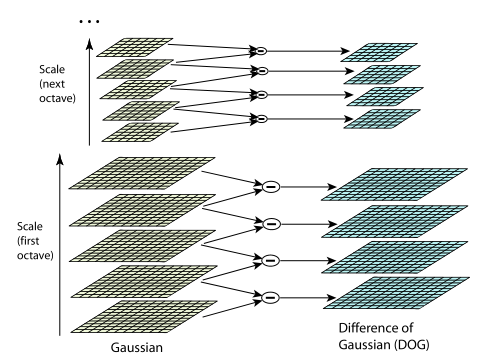
\includegraphics[width=0.6\textwidth]{dog.png}
    \caption{Пирамида Гаусианнов}
    \label{fig:dog1}
\end{figure}

После построения пирамиды разностей гауссианов по всем точкам в пирамиде ищутся локальные экстремумы. Если точка больше (меньше) всех своих 26 соседей (Рис. 2) в пирамиде разностей, то она считается ключевой.

\begin{figure}[h]
    \centering
    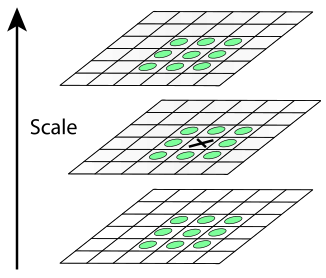
\includegraphics[width=0.5\textwidth]{dog2.png}
    \caption{Локальный экстремум в пирамиде Гауссианов}
    \label{fig:dog2}
\end{figure}

Таким образом мы для исходных изображений разных размеров мы получим ключевые точки (и небольшую область возле них) одного и того же размера - это и даёт инвариантность относительно масштабирования.

Направление ключевой точки вычисляется исходя из направлений градиентов точек, соседних с особой. Все вычисления градиентов производятся на изображении в пирамиде гауссианов, с масштабом наиболее близким к масштабу ключевой точки. Величина и направление градиента в точке $(x,y)$ вычисляются по формулам (3) и (4) соответственно.

\begin{equation}
    m(x,y)=\sqrt{(L(x+1,y) - L(x-1,y))^2 + (L(x,y+1) - L(x,y-1))^2}
\end{equation}
\begin{equation}
    \theta(x,y)=\arctan{\left(\frac{L(x,y+1) - L(x,y-1)}{L(x+1,y) - L(x-1,y)}\right)}
\end{equation}

Направление считается в $\sigma$-окрестности ключевой точки.  Каждая точка окрестности $(x, y)$ вносит вклад и итоговое значение считается за направление ключевой точки.

\subsection{Извлечение дескрипторов}

Как уже говорилось ранее - дескриптор должен очень хорошо и уникально описывать ключевую точку. В общем случае это может быть любой объект, который будет выполнять данные функции и является инвариантным относительно преобразований исходного изображения.

В алгоритме SIFT дескриптор представляет из себя вектор, содержащий информацию об окрестности ключевой точки. Дескриптор вычисляется на том же гауссиане, на котом получен оптимальный размер особой точки. Перед вычислением, для достижения инвариантности относительно поворота изображения всю область ключевой точки поворачивают на угол направления ключевой точки.

\begin{figure}[h]
    \centering
    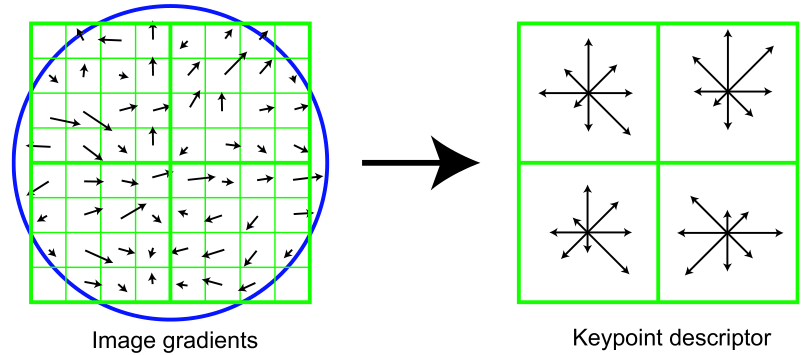
\includegraphics[width=0.8\textwidth]{desc.png}
    \caption{Получение дескриптора}
    \label{fig:desc}
\end{figure}

На Рис.3 показана окрестность ключевой точки (слева) и полученный на её основе дескриптор (справа). Маленькая стрелочка, в центре каждого пикселя в $\sigma$-окрестности обозначает градиент этого пикселя. Круг обозначает окно свертки с гауссовым ядром. Для этого ядра определяется $\sigma$, равное половине ширины окна дескриптора. В дальнейшем значение каждой точки окна дескриптора будет домножаться на значение гауссова ядра в этой точке, как на весовой коэффициент.

Как видно справа дескриптор имеет размерность 2x2x8 (количество регионов по горизонтали, количество регионов по вертикали, количество компонент гистограммы этих регионов). Гистограмма для каждого региона строится в соответствии со значениями градиентов пикселей, входящих в  $\sigma$-окрестность (8 штук):

\begin{enumerate}
    \item Каждая гистограмма так же покрывает участок в 360 градусов и делит его на 8 частей;
    \item В качестве весового коэффициента берется значение гауссова ядра, общего для всего дескриптора;
    \item В качестве ещё одних весовых коэффициентов берутся коэффициенты трилинейной интерполяции;
\end{enumerate}

Каждому градиенту в окне дескриптора можно приписать три вещественные координаты $(x, y, n)$, где $x$ — расстояние до градиента по горизонтали, $y$ — расстояние по вертикали, $n$ — расстояние до направления градиента в гистограмме (имеется ввиду соответствующая гистограмма дескриптора, в которую вносит вклад этот градиент). Коэффициент трилинейной интерполяции определяется для каждой координаты $(x, y, n)$ градиента как $1-d$, где $d$ равно расстоянию от координаты градиента до середины того единичного промежутка в который эта координата попала. Каждое вхождение градиента в гистограмму умножается на все три весовых коэффициента трилинейной интерполяции.

Дескриптор ключевой точки состоит из всех полученных гистограмм. Как уже было сказано размерность дескриптора на рисунке $32$ компоненты (2x2x8), но на практике используются дескрипторы размерности $128$ компонент (4x4x8). Полученный дескриптор нормализуется, после чего все его компоненты, значение которых больше $0.2$, урезаются до значения $0.2$ и затем дескриптор нормализуется ещё раз. В таком виде дескрипторы готовы к использованию.

\section{Анализ других алгоритмов}

SIFT дескрипторы не лишены недостатков. Не все полученные точки и их дескрипторы будут отвечать предъявляемым требованиям. Естественно это будет сказываться на дальнейшем решении задачи сопоставления изображений. В некоторых случаях решение может быть не найдено, даже если оно существует. Например, при поиске аффинных преобразований (или фундаментальной матрицы) по двум изображениям кирпичной стены может быть не найдено решения из-за того, что стена состоит из повторяющихся объектов (кирпичей), которые делают похожими между собой дескрипторы разных ключевых точек. Несмотря на это обстоятельство, данные дескрипторы хорошо работают во многих практически важных случаях. SIFT является наиболее математически обоснованным, но относительно медленным алгоритмом.

\subsection{Дескриптор SURF}

В 2008 был представлен ближайший конкурент SIFT дескриптора, \hyperref[itm:surf]{ SURF [\ref{itm:surf}]} дескриптор. В идейном смысле он похож на своего предшественника, но процедура описания окрестности интересной точки несколько иная, поскольку в ней используются не гистограммы взвешенных градиентов, а отклики исходного изображения на вейвлеты Хаара. Вейвлет — математическая функция, позволяющая анализировать различные частотные компоненты данных. Вейвлет Хаара — один из первых и наиболее простых вейвлетов, обладает компактным носителем, хорошо локализован в пространстве, но не является гладким. 

На первом шаге получения дескриптора вокруг ключевой точки строится квадратная область, которую ориентируют по некоторому предпочтительному направлению. Затем область разделяется на квадратные сектора. В каждом из секторов в точках, принадлежащих регулярной сетке, вычисляются отклики на два вида вейвлетов — горизонтально и вертикально направленные. Отклики взвешиваются Гауссианом, суммируются по каждому сектору, и образуют первую часть дескриптора.

Вторая часть состоит из сумм модулей откликов. Это сделано для того, чтобы учитывать не только факт изменения яркости от точки к точке, но и сохранить информацию о направлении изменения. SURF-дескриптор имеет длину 64. Как и SIFT, SURF-дескриптор инвариантен к аддитивному изменению яркости. Инвариантность к мультипликативному изменению яркости достигается путем нормировки дескриптора. SURF является эвристическим, но и более быстрым, чем SIFT.

\subsection{Дескриптор BRIEF}

Чем меньше длина дескриптора, тем меньше памяти требуется для его хранения, и меньше времени на сравнение его с другими. Эта черта очень важна при обработке большого числа изображений. К наиболее компактным относится дескриптор \hyperref[itm:brief]{ BRIEF [\ref{itm:brief}]}. Для вычисления дескриптора в точке $p$ сравниваются значения яркости точек, расположенных в ее окрестности. При этом сравниваются значения яркости не всех точек со всеми, а анализируется лишь небольшое подмножество соседних пар точек, координаты которых распределены случайно (но одинаковым образом для каждой анализируемой точки $p$). Если яркость в точке $pi_1$ больше, чем яркость в точке $pi_2$, то $i$-я компонента дескриптора принимает значение $1$, в противном случае она становится равной нулю. Фрагмент, по которому вычисляются дескрипторы, предварительно сглаживается. BRIEF-дескрипторы чрезвычайно просты в вычислении, поскольку их значения равны результату сравнения двух чисел. Они также очень компактны, поскольку результат элементарного теста — это число $0$ или $1$, то есть один бит.

В стандартной реализации для построения одного BRIEF-дескриптора требуется выполнить $256$ сравнений, что дает итоговую длину $64$ байта. Это очень мало, учитывая, что SIFT-дескриптор состоит из $128$ действительных чисел, то есть занимает как минимум $512$ байтов. Наконец, сравнение BRIEF-дескрипторов занимает очень мало времени, поскольку сводится к вычислению расстояния Хэмминга между двумя последовательностями битов. Расстояние Хэмминга — число позиций, в которых соответствующие символы двух слов одинаковой длины различны, вычисляется по формуле:

\begin{equation}
    d_{ij} = \sum_{k=1}^{p}|x_{ik} - x_{jk}|
\end{equation}

Эта элементарная операция выполняется чрезвычайно быстро на любом современном процессоре. Сами по себе дескрипторы BRIEF не инвариантны к повороту. Однако такой инвариантности можно добиться, если предварительно повернуть фрагмент вокруг ключевой точки на угол, соответствующий, например, доминирующему направлению градиента яркости, как это делается для дескрипторов SIFT и SURF. Точно так же можно достичь инвариантности к другим ракурсным искажениям.

\subsection{Дескриптор GLOH}

Дескриптор \hyperref[itm:gloh]{ GLOH (Gradient location-orientation histogram) [\ref{itm:gloh}]} является модификацией SIFT-дескриптора, который построен с целью повышения надежности. По факту вычисляется SIFT дескриптор, но используется полярная сетка разбиения окрестности на бины (Рис. 4): 3 радиальных блока с радиусами 6, 11 и 15 пикселей и 8 секторов. В результате получается вектор, содержащий 272 компоненты, который проецируется в пространство размерности 128 посредством использования анализа главных компонент.

\begin{figure}[h]
    \centering
    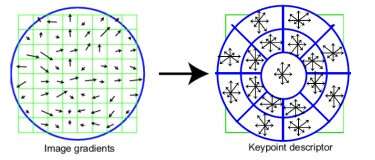
\includegraphics[width=0.8\textwidth]{gloh.jpg}
    \caption{Полярная сетка разбиения на бины}
    \label{fig:gloh}
\end{figure}

\subsection{FAST детектор}

FAST (Features from accelerated segment test - Особенности ускоренных испытаний сегмента) - алгоритм детекции ключевых точек. Детектор считает пиксели в круге Брезенгема (круге построенном с помощью алгоритма Брезенгема построения кривых 2-го порядка) радиуса $r$ вокруг точки кандидата. Если n смежных пикселей ярче чем центр, по крайней мере, в $t$ раз или темнее центра то пиксель под центром считается особенностью. Хотя r в принципе, может принимать любое значение, только значение $r=3$ используется (соответствующий круг 16 пикселей окружности), и тесты показывают, что оптимальное значение $n=9$. Это значение n наименьшее, при котором края не обнаруживаются.

\subsection{Дескриптор ORB}

\hyperref[itm:orb]{ ORB (Oriented FAST and rotated BRIEF) [\ref{itm:orb}]} - ещё один алгоритм соединяющий в себе и дополняющий детектора ключевых точек FAST и бинарных дескрипторов BRIEF. Был предложен Ethan Rublee в 2010 году. Также как и BRIEF, ORB имеет размер 32 байта и для сравнения использует расстояния Хэминга. После детектирования точек с помощью FAST-a ORB выделяет $N$ топ точек используя меру Харисса. Как следует из названия, далее ORB ориентирует найденные ключевые точки. Так как BRIEF плохо работает с поворотом, ORB исправляет это с помощью ориентации, полученной на предыдущем шаге.

\section{Выводы}

В этой главе мной были рассмотрены основные алгоритмы компьютерного зрения с помощью которых можно доставать и сравнивать ключевые точки. Подводя итог анализа: SIFT самый первый, математически точный и медленный дескриптор, на котором основаны большинство современных эвристических алгоритмов feature extraction.

В своих дальнейших исследованиях я буду использовать SIFT - так как он является стандартом в компьютерном зрении. SURF - запатентован в США и является закрытым, также авторы BRIEF приводят результаты экспериментов в которых при одинаковых условиях на некоторых тестовых изображениях точность детектирования с помощью BRIEF почти в $1.5$ раза выше, чем с использованием SURF-дескрипторов.

Очень привлекательным выглядит ORB - он быстрый, устойчивый и действительно является эффективность альтернативой SIFT'у. Также он совершенно бесплатный и свободно распространяемый. Поэтому я решил остановить выбор на нём, а SIFT использовать как точное значения и для анализа результатов разными средствами. OpenCV предоставляет удобный интерфейс создания дескрипторов и детекторов, что даёт возможность динамически сменять features methods. Практические эксперименты и их результаты будут рассмотрены в следующей главе.

\newpage